\originalchapter{15.053 作业题与解答}\label{ass:15053-homework}
本章按2013年课程的八份作业版本逐题整理. 作业1、2的两个版本共用前两题, 因而只写一次; 第三题分别保留组1与组2. 去重后有24道主问题、104个第一层作答块; 整题无子问时计一块, 同一(c)下的(i)--(vi)仍是一个第一层块. 作业3的题目数据与唯一官方解答来自电子表格, 已实际读取其六张工作表, 不是根据PDF中的“见工作簿”猜补.

题面采用数学条件与数据的中文重述. 凡原题说明取自外部教材, 保留原课程题号及出处关系, 不重译外书叙事. 解答以官方解答为对照重构, 其错误、遗漏与独立补证均在相应题中标明. 原题中的连续产量按线性规划处理; 若要整数产量, 必须另加整数条件. 数值建模题由\texttt{tools/audit\_lp\_homework.py}实际计算, 可行性、对偶界、精确换基及枚举结果留在源码审读记录中.

\originalsection{作业1：变量、变换与产品组合}
原交期为2013年2月12日. 官方资源的组1文件对应姓氏首字母A--H, 组2对应I--Z; 组1题面页首误印“Second Group”, 官方解答又误印A--F. 这里以资源版本与实际第三题内容建立映射, 不据这些错字重分组.

\begin{exercise}\label{ass:15053-ps1-q1}
作业1第1题（两组共用）. 三种保护套依次为iPod、iPhone、iPad. 全部产线用于单一产品时, 日产量依次为6000、5000、3000件; 每周5个工作日, 每日8小时. 每件仓储体积为0.04、0.045、0.21立方英尺, 总仓储上限6000. 周最低产量为5000、0、4000件, 周最高需求为10000、15000、8000件; 单件利润为4、6、10美元.

(a) 说明线性假设, 用每天生产三产品的时间比例$x_1,x_2,x_3$建模并说明各约束. (b) 改用周产量$y_1,y_2,y_3$建模. (c) 改用一周iPod生产小时$z_1$、iPhone生产小时$z_2$和全部生产小时$z_3$建模, 目标单位为千美元. (d) 写出$z$与$x$的关系. (e) 按工作簿以千件为产量单位求解. (f) 推广到$n$种产品: $x_j$为生产天数, $p_j$为日产量, $P$为周生产天数, $s_j$为单位体积, $S$为仓储上限, $r_j$为单位利润, $b_j,d_j$为最低与最高需求, 写代数模型.
\end{exercise}
\begin{solution}
官方解答重构并修正单位与约束. (a) 假设产量与生产时间成正比, 允许分数时间, 没有切换损耗, 所有产量均售出. 模型为
\begin{align*}
\max\;&120000x_1+150000x_2+150000x_3,\\
&x_1+x_2+x_3\le1 &&\text{（时间）},\\
&1200x_1+1125x_2+3150x_3\le6000&&\text{（仓储）},\\
&5000\le30000x_1\le10000,\quad0\le25000x_2\le15000,\\
&4000\le15000x_3\le8000&&\text{（最低产量与需求上限）}.
\end{align*}
(b) 目标为$4y_1+6y_2+10y_3$, 时间约束为$y_1/6000+y_2/5000+y_3/3000\le5$, 仓储约束为$0.04y_1+0.045y_2+0.21y_3\le6000$, 并加给定产量上下界. 官方(b)把第三项误写为$y_1/3000$, 应为$y_3/3000$.

(c) iPad生产时间是$h=z_3-z_1-z_2$. 要求$z_1,z_2,h\ge0$, $z_3\le40$. 周产量是$(750z_1,625z_2,375h)$, 因而目标为$3z_1+3.75z_2+3.75h$（千美元）, 仓储为$30z_1+28.125z_2+78.75h\le6000$, 产量上下界分别代入这三个产量. 官方列式遗漏总时间上限, 且目标未换成千美元, 这里补正. (d) $z_1=40x_1$, $z_2=40x_2$, $z_3=40(x_1+x_2+x_3)$.

(e) 工作簿把iPod最低产量改为恰好5千件, 与(b)的下界不同; 两者的最优值相同. 一组最优千件产量是$(5,7.5,8)$, 利润145000美元, 与官方工作簿一致; 另一组是$(5,85/6,4)$. 证明最优可观察每个生产日的利润分别为24000、30000、30000美元, 而iPod至少占$5/6$天, 所以利润不超过$30000\cdot5-6000\cdot(5/6)=145000$. 两组都达到上界. 因而最优产量不唯一, 不应把不同求解器输出视为错误.

(f) $\max\sum_{j=1}^nr_jp_jx_j$, 约束$\sum_jx_j\le P$, $\sum_js_jp_jx_j\le S$, $b_j\le p_jx_j\le d_j$, $x_j\ge0$.
\end{solution}

\begin{exercise}\label{ass:15053-ps1-q2}
作业1第2题（两组共用）. 判断能否严格改写为单个线性规划, 能时写出模型, 不能时指出障碍, 不要求求解.

(a) $x_1,x_2$自由, 最小化$\max\{2.3x_1+x_2,4.3x_1-0.5x_2,2.5x_1+3.5x_2\}$, 约束$x_1/(x_1+x_2)\le0.5$, $10x_1+28x_2=3.4$, $x_1+x_2\ge0$. (b) 最小化$|0.8x_1+0.9x_2|$, 约束$|0.9x_1+1.2x_2|\le10$, $x_1\ge0$, $x_2$自由.
\end{exercise}
\begin{solution}
(a) AI独立修正官方解答. 比例本身要求$x_1+x_2\ne0$, 与给定非负条件合起来是严格正. 在此域上可以交叉乘得到$x_1\le x_2$, 并引入$t$满足$t\ge2.3x_1+x_2$, $t\ge4.3x_1-0.5x_2$, $t\ge2.5x_1+3.5x_2$. 但严格正条件不是普通LP的闭线性不等式.

由等式$x_2=(3.4-10x_1)/28$, 原可行域恰为$-17/90<x_1\le17/190$. 若仅保留$x_1+x_2\ge0$, 会错误地加入$(-17/90,17/90)$, 其比例未定义. 在这个区间, 三个仿射函数的最大者始终是第三个, 它等于$0.425+1.25x_1$. 所以原问题的下确界是$17/90$, 但不取到; 官方闭LP却在新增点取到该值. 任何非空且目标有有限下界的普通LP都取到最小值, 故这不是严格等价的LP改写. 若明示采用零投放处的扩展定义, 上述闭LP可作为修改后的问题, 不能称原题的等价模型. 官方第三个上图约束还误用了反向不等号.

(b) 官方解答重构. 最小化$t$, 加$t\ge0.8x_1+0.9x_2$, $t\ge-0.8x_1-0.9x_2$, $-10\le0.9x_1+1.2x_2\le10$, 保留原变量符号条件. 正确最小化方向使$t$在最优处等于绝对值.
\end{solution}

\begin{exercise}\label{ass:15053-ps1-q3-g1}
作业1第3题, 组1：混合配料（原课程注明据\emph{Applied Mathematical Programming}第1章第11题）. 原料A、B、C、D的日供应上限为$(4000,5000,3500,5500)$加仑, 单位成本为$(0.60,0.52,0.48,0.35)$美元. 制成Deluxe、Standard、Economy, 数学数据如下.
\begin{center}\begin{tabular}{lrrrr}\toprule
成品&A最大比例&C最小比例&D最大比例&售价\\\midrule
Deluxe&0.60&0.20&0.10&7.9\\
Standard&0.15&0.60&0.25&6.9\\
Economy&无&0.50&0.45&5.0\\\bottomrule
\end{tabular}\end{center}
(a) 建立利润最大LP. (b) 按工作簿求最优配料与利润. (c)(i) 求Economy值得生产的最低售价（精确至5美分）; 原题此处错写Deluxe, 按前句及官方解答保留Economy的实际意图. (ii) 分别删去三成品的D最大比例约束, 哪一条最有价值? 原题后一句错写A, 按前句D说明讨论. (iii) Deluxe售价改为7.95、8.00、8.05时, 分别求利润增量. (iv) 预测并验证涨价5\%时的利润; 对1\%--10\%涨价写出利润公式. (v) 用原基公式预测售价8.5时的增量, 再实际求解, 找原公式有效的最高售价（精确至5美分）. (vi) 能否多买少量A, 最高可接受购买价是多少? (d) 推广到$n$种原料、$m$种成品: 售价$p_j$, 成本$c_i$, 供应$a_i$, 成分比例下界$r_{ij}$及上界$q_{ij}$, 写代数模型.
\end{exercise}
\begin{solution}
官方解答重构, 数值与有效范围由AI独立验算. (a) 令$x_{ij}\ge0$为投入成品$j$的原料$i$加仑数, $T_j=\sum_i x_{ij}$. 目标为$\max\sum_{ij}(p_j-c_i)x_{ij}$, 供应约束为$\sum_jx_{ij}\le a_i$. 比例直接写为$x_{Aj}\le q_{Aj}T_j$, $x_{Cj}\ge r_{Cj}T_j$, $x_{Dj}\le q_{Dj}T_j$, 其中Economy无A上限. $T_j=0$时表示不生产该成品, 所有配料也为0; 这种质量比例的零产量约定须说清, 无须写未定义的$0/0$.

(b) 最优配料矩阵（行依次A--D, 列依次三成品）为
\[
X=\begin{pmatrix}4000&0&0\\4750&250&0\\2500&1000&0\\1250&1250/3&0\end{pmatrix}.
\]
成品为$(12500,5000/3,0)$, 利润$308960/3=102986.6667$. 所有供应与成分约束直接代入可核. 实际求解同时给对偶上界同值, 完整乘子及残差在计算记录中.

(c)(i) 最低临界售价为$1619/312=5.1891026$美元, 按5美分精度报约5.20. 在临界点有包含Economy的同值最优方案, 超过临界点可提高利润. 一种竞争方案的成品量为$(216250/17,0,32500/17)$; 将它与(b)方案的利润作比较即得该临界值, 全部LP约束及对偶价格验证其为阈值.

(ii) 分别删除Deluxe、Standard、Economy的D上限, 利润依次为129945、104903.3333、103402.1429, 因而删除Deluxe的上限最有价值. (iii) 增量依次为625、1250、1875, 因为相应范围内Deluxe产量保持12500.

(iv) 原基公式不是对全部1\%--10\%有效. 设新售价为$p$, 则在本题所问范围内
\[
V(p)=\begin{cases}
308960/3+12500(p-7.9),&7.9\le p\le8.21,\\
(125000p-64495)/9,&8.21\le p\le8.69.
\end{cases}
\]
第二段用完A、B、C, 全部用于Deluxe, D投入$12500/9$, 总Deluxe为$125000/9$. 两段交于8.21; 逐段的可行配料及非负对偶证书也给全局最优, 不能仅按短区间线性外推. 涨价5\%使$p=8.295$, 实际利润$972380/9=108042.2222$, 增量5055.5556. 原题“可假设1\%--10\%”与单一基公式有效范围不一致, 这里给完整分段结果.

(v) 原公式预测增加7500; 实际利润110889.4444, 增加7902.7778. 精确最高有效售价8.21（按题目精度约8.20）. (vi) 增加A一加仑后的利润102994.6731, 增量8.0064103, 已扣原成本0.60. 所以少量新A的总购买价低于$8.6064103$美元/加仑时有净收益, 等号时无净增益. 官方把基准利润写成102903等数, 这里按同一模型重算.

(d) 目标为$\max\sum_{i=1}^n\sum_{j=1}^m(p_j-c_i)x_{ij}$; 约束$\sum_jx_{ij}\le a_i$, $r_{ij}\sum_kx_{kj}\le x_{ij}\le q_{ij}\sum_kx_{kj}$, $x_{ij}\ge0$. 无成分限制时相应取$r_{ij}=0$, $q_{ij}=1$.
\end{solution}

\begin{exercise}\label{ass:15053-ps1-q3-g2}
作业1第3题, 组2：电子产品测试（原课程注明据Heizer与Render, \emph{Operations Management}, 2010, B.29）. 六产品依次为内置调制解调器I、外置调制解调器E、电路板C、USB存储U、硬盘H、扩展内存M. 每件在三设备上测试所需分钟为
\[
Q=\begin{pmatrix}7&3&12&6&18&17\\2&5&3&2&15&17\\5&1&3&2&9&2\end{pmatrix}.
\]
三设备每周可用小时为$(130,130,100)$, 小时人工费为$(16,12,18)$美元. 产品售价为$(200,120,180,130,430,260)$, 材料成本为$(35,25,40,45,170,60)$, 需求上限为$(2000,1500,1800,1200,1000,1000)$.

(a) 写利润最大LP. (b) 按工作簿求最优方案. (c)(i) 三设备增加一分钟各值多少, 应增加哪种设备时间? (ii) 设备2每周时间改为131、132、133小时时, 分别求增量. (iii) 预测并验证135小时的增量, 写130+$t$小时、$1\le t\le10$时的公式. (iv) 预测150小时增量并实际求解; 找该公式最长有效增量范围（精确至一小时）. (v) 人工费改为$(18,13,20)$时, 最优方案如何改变? (vi) 单独改变设备3人工费, 原生产组合保持最优的范围是什么（精确至一美元）? (d) 用产品数$m$、设备数$n$、设备小时$a_i$、人工费$c_i^L$、材料成本$c_j^M$、售价$r_j$、需求上限$b_j$和测试分钟$q_{ij}$写代数模型. 原题把$b_j$误称材料可用量, 依数据及官方模型保留其需求上限含义.
\end{exercise}
\begin{solution}
官方解答重构, 灵敏度范围由AI独立修正. (a) 令$x_j$为产品周产量, 单位净利润为$c_j=r_j-c_j^M-\sum_i c_i^Lq_{ij}/60$. 模型为$\max c\T x$, $Qx\le(7800,7800,6000)\T$, $0\le x\le b$. 工作簿的电路板单位利润缓存值138.9333与当前数据不符, 按数据应为$140-(16\cdot12+12\cdot3+18\cdot3)/60=135.3$, 本稿据题面与表中输入重算.

(b) $x_I=15600/29=537.9310$, $x_E=39000/29=1344.8276$, 其余0, 利润211666.8966. 前两设备满负荷, 第三设备剩余1965.5172分钟. 对偶价格（美元/分钟）为$(21.3919540,5.7448276,0)$; 加权后的每产品资源价格至少为净利润, 候选方案达到上界, 所以最优. 官方解答PDF(b)的混料利润提示102986.7误植, 题面与工作簿对应本题的211666.9.

(c)(i) 增加一分钟依次增加21.3919540、5.7448276、0美元. 未计购置费时设备1时间最有价值, 是否实际购买还要比较成本. (ii) 增量依次344.6896552、689.3793103、1034.0689655. (iii) 135小时增量1723.4482759; $V(t)=211666.8965517+344.6896552t$. 同一基的产量为$x_I=(15600-180t)/29$, $x_E=(39000+420t)/29$.

(iv) 150小时即$t=20$, 线性公式预测6893.7931, 实际只增加3693.1034. 上式有效至$t=75/7=10.7142857$小时, 此时外置产品达到1500件上限; 按整数小时报告10小时. 再增加设备2时间, 原六产品模型的最优利润为215360, 不再增加. (v) 生产组合不变, 利润降为211142.4138.

(vi) 令设备3小时人工费为$h$. 保持I、E为正基本产品时, 前两设备价格由两产品净利润方程给出
\[
\pi_1=9409/435-23h/1740,\qquad \pi_2=821/145+2h/435.
\]
其余四产品的检验数依次为$11(h-1480)/116$, $(16h-25275)/435$, $(11h-128800)/580$, $(197h-473100)/1740$. 要求$\pi_1,\pi_2\ge0$且这些检验数非正, 得数学范围$-1231.5\le h\le1480$; 人工费非负时为$0\le h\le1480$. 等号1480处可能出现其他同值组合, 原组合仍最优. 官方“所有工资率均稳定”不正确.

(d) $\max\sum_{j=1}^m(r_j-c_j^M-\frac1{60}\sum_{i=1}^nc_i^Lq_{ij})x_j$, 约束$\sum_jq_{ij}x_j\le60a_i$, $0\le x_j\le b_j$.
\end{solution}

\originalsection{作业2：图解、单纯形与重新定价}
原交期为2013年2月21日. 两组第三题使用作业1的另一组模型, 但均修改参数, 因而须分别求解.

\begin{exercise}\label{ass:15053-ps2-q1}
作业2第1题（两组共用）. 考虑$\max(x_1+2x_2)$, 约束$x_1-x_2\ge-2$, $x_1+x_2\le4$, $x_1\le2.5$, $x_2\le3$, $x_1,x_2\ge0$.

(a) 画可行域, 判断是否无界. (b) 哪些约束冗余? (c) 用图解法求最优解并说明方法. (d) 最优解是否唯一, 若不唯一给两个, 若唯一说明图形理由. (e) 加入$2x_1+x_2\ge\alpha$, 分别求它冗余、原最优解不再最优、问题不可行的$\alpha$范围. (f) 改目标为$x_1+\beta x_2$, 求$(2.5,1.5)$最优的$\beta$范围.
\end{exercise}
\begin{solution}
官方解答重构并补足唯一性. (a) 可行域是下图五边形, 顶点为$(0,0),(2.5,0),(2.5,1.5),(1,3),(0,2)$, 故有界.
\begin{center}\begin{tikzpicture}[x=1.2cm,y=1cm]
\fill[structurecolor!8] (0,0)--(2.5,0)--(2.5,1.5)--(1,3)--(0,2)--cycle;
\draw[->] (-.2,0)--(3.2,0) node[right]{$x_1$};\draw[->] (0,-.2)--(0,3.7) node[above]{$x_2$};
\draw[thick] (0,0)--(2.5,0)--(2.5,1.5)--(1,3)--(0,2)--cycle;
\fill (1,3) circle(1.5pt) node[above right]{$(1,3)$};\node[right] at (2.5,1.5){$(2.5,1.5)$};
\node[left] at (0,2){$2$};\node[below] at (2.5,0){$2.5$};
\end{tikzpicture}\end{center}
(b) 前两约束相加给$2x_2\le6$, 故$x_2\le3$冗余. 其他三条及两条非负约束各有不受其他约束蕴含的边界.

(c) 将等利润直线向目标增大方向平移, 最后接触$(1,3)$, 最优值7. 也可将$x_1+x_2\le4$乘$3/2$, 将$-x_1+x_2\le2$乘$1/2$, 得$x_1+2x_2\le7$. (d) 达到该界必须让两条不等式同时等号, 唯一交点为$(1,3)$, 所以唯一; 图形上目标线不与相邻边平行.

(e) $2x_1+x_2$在原可行域的最小值0、最大值6.5, 原最优点值5. 因而新增约束在$\alpha\le0$时冗余; 原最优点在$\alpha>5$时被排除, 其中$5<\alpha\le6.5$仍有别的可行方案; $\alpha>6.5$时不可行. (f) $(1,\beta)$是$(1,0)$与$(1,1)$的非负组合恰当且仅当$0\le\beta\le1$, 这正是该顶点活跃约束的法向锥. 两端允许整条相邻边同值.
\end{solution}

\begin{exercise}\label{ass:15053-ps2-q2}
作业2第2题（两组共用; 原课程注明据\emph{Applied Mathematical Programming}第2章第6题）. 三轮胎每件利润为6、4、8美元, 每100件在成型、硫化、装配三工序所需小时分别为矩阵
\[
A=\begin{pmatrix}2&2&4\\3&2&2\\2&1&2\end{pmatrix},\qquad b=(12,14,16)\T.
\]
(a) 建LP, 假设全部售出. (b) 补齐工作簿中的初表, 用单纯形法给出到最优表的换基序列. (c)(1) 给初始产量与全部松弛; (2) 给最优产量与利润. (d)(i) 成型从12增至13小时的利润增量; (ii) 装配从16增至17小时的增量; (iii) 讨论影子价格与松弛的关系（原题附加分）.
\end{exercise}
\begin{solution}
官方解答重构并修正互补松弛的逆命题. (a) 令$x$以100件为单位, $\max(600x_1+400x_2+800x_3)$, $Ax\le b$, $x\ge0$. 若以件为单位, 将时间系数除100并采用原利润系数即可.

(b) 初始表用松弛$s_1,s_2,s_3$为基. 先让$x_3$进入、$s_1$离开, 得
\[
x_3=3-\tfrac12x_1-\tfrac12x_2-\tfrac14s_1,\quad
s_2=8-2x_1-x_2+\tfrac12s_1,\quad s_3=10-x_1+\tfrac12s_1,
\]
且$z=2400+200x_1-200s_1$. 再让$x_1$进入、$s_2$离开, 得最优字典
\begin{align*}
x_1&=4-\tfrac12x_2+\tfrac14s_1-\tfrac12s_2,\\
x_3&=1-\tfrac14x_2-\tfrac38s_1+\tfrac14s_2,\\
s_3&=6+\tfrac12x_2+\tfrac14s_1+\tfrac12s_2,\\
z&=3200-100x_2-150s_1-100s_2.
\end{align*}
所有非基本变量检验数非正, 所以已最优. 实际脚本还采用Bland合法序列, 两种序列得到同值最优解.

(c)(1) 初始产量全0, 松弛为$(12,14,16)$. (2) 产量为400、0、100件, 松弛为$(0,0,6)$小时, 利润3200. (d)(i) 同一最优基在增加一小时成型时间后仍可行, $x_1=4.25,x_3=0.625$, 利润增加150. (ii) 装配原有6小时闲置, 增加一小时无收益. (iii) 非零松弛强制相应非负对偶价格为0; 正影子价格强制约束活跃. 活跃约束的价格仍可能为0, 官方“活跃约束必有非零价格”的一般断言不成立.
\end{solution}

\begin{exercise}\label{ass:15053-ps2-q3-g1}
作业2第3题, 组1. 使用习题\ref{ass:15053-ps1-q3-g2}的电子测试数据, 将三人工费改为$(18,15,12)$. 新增外置硬盘, 每件售价127、材料成本50美元, 三测试时间为$(3,2,6)$分钟, 不设需求上限.

(a) 求最优利润与产量. (b) 新外置硬盘在最优组合中为0, 售价至少增加多少才值得生产（精确至一美元）? (c) 设备2可用小时改为130+$t$, $t=1,2,3$, 求利润增量. (d) 估计并验证140小时利润, 写$1\le t\le10$的公式. (e) 预测150小时的增量并实际求解, 找公式最长有效增量范围（精确至一小时）.
\end{exercise}
\begin{solution}
官方解答重构并独立修正错字与精度. (a) 原六产量为$(15600/29,39000/29,0,0,0,0)$, 新产品0, 利润211420.3448. 官方两项都写$x_E$, 正确分别是I与E. 对偶价格为$(21.4379310,5.6672414,0)$美元/分钟.

(b) 新产品净利润为$127-50-(18\cdot3+15\cdot2+12\cdot6)/60=74.4$. 按资源价格计的成本为$3\pi_1+2\pi_2=75.6482759$, 故售价的临界增加为1.2482759美元, 临界售价128.2482759; 若只按整数美元报价则要129. 临界价处可有正生产的同值最优组合, 再提高才能严格改善利润.

(c) 增量为340.0344828、680.0689655、1020.1034483. 官方第一项340.3451为误植. (d) 140小时利润214820.6897, 增量3400.3448; 公式$V(t)=211420.3448276+340.0344828t$. 基本产量变化与习题\ref{ass:15053-ps1-q3-g2}(c)(iii)相同. (e) 150小时公式预测增加6800.6897, 实际利润217612.5, 增量6192.1552; 此时原I、E和新外置硬盘的产量为$(262.5,1500,487.5)$. 原公式精确有效至$t=75/7$小时, 按整数小时为10小时.
\end{solution}

\begin{exercise}\label{ass:15053-ps2-q3-g2}
作业2第3题, 组2. 使用习题\ref{ass:15053-ps1-q3-g1}的原料与成分数据, 售价改为$(7.7,6.8,4.9)$, 且Deluxe日产量不超过12000加仑.

(a) 求利润与最优配料. (b) Economy的最低值得生产售价是多少（精确至5美分）? (c) Standard售价改为$6.8+s$, $s=0.05,0.10,0.15$, 求利润增量. (d) 预测Standard售价7.2时利润, 写$0.05\le s\le0.25$的公式. (e) 用该公式预测售价7.5的增量, 实际求解核对.
\end{exercise}
\begin{solution}
官方解答重构并独立修正算术. (a) 一组最优配料为
\[
X=\begin{pmatrix}3675&0&0\\4725&275&0\\2400&1100&0\\1200&1375/3&0\end{pmatrix},
\quad T=(12000,5500/3,0),\quad V_0=97801.25.
\]
配料不唯一: 在不违反供应和比例的范围内, A、B可在两种成品之间等量互换, 总成本与成品量不变. 实际求解输出的另一矩阵及对偶上界也已核对.

(b) 精确阈值5.70625美元, 按5美分精度可报约5.70或5.75. 例如含2200加仑Economy且无Standard的竞争方案, 在该售价处与原方案同值; 对偶检验亦给相同阈值. (c) 增量分别$275/3=91.6667$, $550/3=183.3333$, 275. (d) $V(s)=97801.25+(5500/3)s$, 所问区间原成品量不变. 售价7.2即$s=0.4$, 实际仍适用, 利润98534.5833. (e) $s=0.7$, 增量1283.3333, 实际利润99084.5833, 公式仍正确. 官方把1283.3333误写为12.8334, 此处按真实模型验证.
\end{solution}

\originalsection{作业3：两阶段法、退化与参数表}
原交期为2013年2月28日. 全部题原要求电子表格提交; 这里把工作簿中的矩阵、参数与答案完整转写为可阅读的数学问题. 单纯形表统一按$-z+\sum_j\bar c_jx_j=\text{RHS}$读取, 正$\bar c_j$才表示极大问题的改善方向.

\begin{exercise}\label{ass:15053-ps3-q1}
作业3第1题. 原问题为
\[
\max(x_1+2x_2+2x_3-3x_4),\quad
\begin{pmatrix}1&6&1&-1\\2&-4&2&-4\\4&0&1&1\end{pmatrix}x=
\begin{pmatrix}8\\4\\6\end{pmatrix},\quad x\ge0.
\]
给三等式分别加人工变量$y_i\ge0$, 第一阶段最大化$-y_1-y_2-y_3$. 完成第一阶段换基, 给其最优基本可行解; 再恢复原目标, 给原问题最优基本可行解.
\end{exercise}
\begin{solution}
官方电子表格解答重构并补精确值. 第一阶段可得到$x=(5/6,3/4,8/3,0)$, $y=(0,0,0)$, 辅助值0; 基为$x_1,x_2,x_3$. 从人工基依次让$x_1,x_3,x_2$进入并让$y_3,y_2,y_1$离开即可达到此基. 人工目标不超过0, 故已经最优且原问题可行.

删去人工列, 恢复原目标, 让$x_4$进入、$x_1$离开, 得$x=(0,7/11,56/11,10/11)$, 值$96/11=8.7272727$. 原矩阵乘此向量恰等于右端. 最优等式对偶乘子为$(8/11,13/22,1/11)$, 满足$A\T\pi\ge(1,2,2,-3)\T$, 且$b\T\pi=96/11$, 所以最优. 官方答案栏把$z$四舍五入到8.7, 不能用它替代精确值.
\end{solution}

\begin{exercise}\label{ass:15053-ps3-q2}
作业3第2题. 对下面退化例使用Bland规则, 求最优基:
\[
z=3-20x_1+\tfrac34x_2-6x_3+\tfrac12x_4,
\quad
\begin{pmatrix}-8&1/4&9&-1&1&0&0\\-12&1/2&3&-1/2&0&1&0\\0&0&0&1&0&0&1\end{pmatrix}
\begin{pmatrix}x_1\\x_2\\x_3\\x_4\\s_1\\s_2\\s_3\end{pmatrix}=\begin{pmatrix}0\\0\\2\end{pmatrix},
\]
所有变量非负, 初始基为$s_1,s_2,s_3$. 基编号把$s_1,s_2,s_3$依次视为5、6、7.
\end{exercise}
\begin{solution}
官方工作簿解答重构并独立精确换基. 此例与第\ref{chap:12}章例\ref{ex:lp-cycle}的循环数据同型: 四列交换为旧$(x_2,x_1,x_4,x_3)$, 第三右端由1改为2. 因此保留新数据, 不直接照搬旧最优产量.

Bland基序列为$(5,6,7)\to(2,6,7)\to(2,1,7)\to(2,4,7)\to(2,4,3)\to(2,4,5)$. 前三次是零步长, 后两次允许正步长. 最优产量$x_2=x_4=2$, $s_1=3/2$, 其余0, 目标为$11/2$. 最终非基本变量$x_1,x_3,s_2,s_3$的检验数分别为$-2,-21/2,-3/2,-5/4$, 给最优证书. 脚本实际以有理数完成五次主元, 无循环.
\end{solution}

\begin{exercise}\label{ass:15053-ps3-q3}
作业3第3题. 每部分从下表重新开始, 只改变一个单元格的值, 使要求成立; 多解时任取一解. 正数统一用$+1$. 列G--M对应$x_1,\ldots,x_7$, 列P为右端, 行11为目标, 行12--14为约束; 当前基为$x_5,x_6,x_7$.
\[
\begin{array}{c|rrrrrrr|r}
 &x_1&x_2&x_3&x_4&x_5&x_6&x_7&\text{P}\\\hline
11\ (-z)&-12&-5&-3&-20&0&0&0&-120\\
12&7&4&-3&-4&1&0&0&8\\
13&-1&1&2&-3&0&1&0&4\\
14&4&-3&0&-1&0&0&1&3
\end{array}
\]
(a) 当前解最优, 且一条边也最优. (b) 当前解最优, 且存在最优射线. (c) 当前解不最优, 下次主元使$x_5$非基本. (d) 当前解不最优, 下次主元使$x_3$基本. (e) 当前解退化. 对(f)、(g)先将P13的4改为0, 再改变一个单元格: (f) 基不最优且下次换基退化, 点不变; (g) 基不最优且下次换基非退化, 点改变.
\end{exercise}
\begin{solution}
官方答案重构并逐项检验. (a) 改G11为0, 令$x_1$沿零检验数方向增加, 比值为$8/7$与$3/4$, 可到下一不同顶点, 整条线段同值. (b) 改J11为0; $x_4$列的三个约束系数均负, 可无限增加, 目标不变. (c) 改H11为1, $x_2$进入, 正比值$8/4=2$, $4/1=4$, 所以$x_5$离开. (d) 改I11为1, $x_3$进入, 唯一正限制为$x_6=4-2x_3$, 因而$x_6$离开. (e) 改P12为0, 一个基本变量为0即可.

(f) 改I11为1, $x_3$进入时行13的比值为$0/2=0$, 产生退化换基. (g) 改G11为1, $x_1$列在零右端行13的系数为负, 该行不限制正步长; 行14给$3/4$, 是非退化步长. 官方工作簿说明另写“把P14的1改为0”, 但原初表P14实际为3且PDF明确指定P13的4. 本稿按PDF题面作答并保留这一版本冲突, 不混改两处.
\end{solution}

\begin{exercise}\label{ass:15053-ps3-q4}
作业3第4题. 所有变量非负, 参数表为
\[
\begin{array}{c|rrrrrrr|r}
 &x_1&x_2&x_3&x_4&x_5&x_6&x_7&\text{右端}\\\hline
-z&0&-2&A&B&0&C&0&-8\\
x_1&1&-2&-1&4&0&1&0&4\\
x_7&0&0&D&0&0&E&1&2\\
x_5&0&1&-3&5&1&0&0&F
\end{array}
\]
每部分给尽可能完整、简洁的条件. (a) 何时当前解可行且不退化? (b) 何时可行且退化? (c) 假设可行且不退化, $A,B,C$满足什么条件使当前解最优? (d) 在(a)、(c)条件下, 给多最优解的附加条件. (e) 假设可行且不退化, 何时当前解是唯一最优解? (f) 假设$A,B\le0$, 什么$C,E$条件使$x_6$进入时$x_7$有资格离基? (g) 什么$A,D$条件使算法可立即证明目标向上无界? (h) 在(a)、(c)条件下, 何时有最优射线?
\end{exercise}
\begin{solution}
官方工作簿解答重构, (f)、(h)由AI独立修正与补全. 初始基本值为$(4,2,F)$. (a) $F>0$. (b) $F=0$. (c) $A,B,C\le0$. 因不退化, 任何正检验数都允许小正步长改善目标, 因而这也必要.

(d) $A,B,C$至少一个为0. 非退化保证沿该非基本变量方向有正可行步长, 即得到不同的同值点. (e) $A,B,C<0$: 目标式$z=8-2x_2+Ax_3+Bx_4+Cx_6$迫使所有非基本变量为0; 反之任一零检验数都给另一最优点.

(f) 要成为改善的进入变量须$C>0$. 正比值来自$x_1$的4及$x_7$的$2/E$, 后者有资格当最小比值恰当且仅当$E\ge1/2$. 等号时并列可选$x_7$; 若指定Bland离基则会选择编号更小的$x_1$. 官方写$C\le0$与进入方向相反, 是错误.

(g) $A>0$, $D\le0$, 且当前基可行（即$F\ge0$）. $x_3$列为$(-1,D,-3)\T$, 无正系数限制步长, 目标随$x_3$无限增加. 原题只要求$A,D$, 但从当前表直接用原始单纯形作无界证书须保留可行性前提.

(h) 完整条件为
\[
A=0\quad\text{且}\quad\bigl[D\le0\ \text{或}\ (C=0\ \text{且}\ D+E\le0)\bigr].
\]
证明: 最优射线的非基本方向满足$d_2=0$, 且只可支持于$A,B,C$中为0的列. 第一行给$-d_3+4d_4+d_6\le0$, 第三行给$-3d_3+5d_4\le0$, 故非零射线必须$d_3>0$, 从而$A=0$. 若$D\le0$, 取纯$x_3$方向即可. 若$D>0$, 第二行$Dd_3+Ed_6\le0$要求$E<0$, $d_6>0$, 因而$C=0$; 又$d_6\le d_3$, 必须$D+E\le0$. 反过来取$d_3=d_6=1,d_4=0$满足这时所有限制. 官方只给$A=0,D\le0$, 是充分条件但漏了组合射线.
\end{solution}

\originalsection{作业4：灵敏度报告与零和博弈}
原交期为2013年3月7日; 原作业无电子表格提交.

\begin{exercise}\label{ass:15053-ps4-q1}
作业4第1题（原课程注明据\emph{Applied Mathematical Programming}第3章第1题; 此处独立重述数学模型与问题）. 三产品依次为椅、凳、桌, 连续产量为$x$, 最大化$3x_1+3x_2+5x_3$, 资源为
\[
\begin{pmatrix}1.2&1.7&1.2\\0.8&0&2.3\\2&3&4.5\end{pmatrix}x\le
\begin{pmatrix}1000\\1200\\2000\end{pmatrix},\quad x\ge0.
\]
三资源依次为弯管小时、焊接小时、金属管磅数. 已给最优产量$(700,0,400/3)$, 利润$8300/3$, 焊接松弛$1000/3$, 其余资源松弛0. 灵敏度报告如下; $\infty$是原表的极大数标记$10^{30}$.
\begin{center}\begin{tabular}{lrrrrr}\toprule
产品&检验数&目标系数&允许增加&允许减少\\\midrule
椅&0&3&2&$7/9$\\
凳&$-83/60$&3&$83/60$&$\infty$\\
桌&0&5&1.75&2\\\bottomrule
\end{tabular}\quad
\begin{tabular}{lrrrr}\toprule
资源&影子价格&右端&允许增加&允许减少\\\midrule
弯管&$7/6$&1000&200&$1400/3$\\
焊接&0&1200&$\infty$&$1000/3$\\
材料&$4/5$&2000&$5000/9$&$1000/3$\\\bottomrule
\end{tabular}\end{center}
(a) 给最优组合与利润. (b) 三资源各增加一单位值多少, 并仅看焊接松弛猜其影子价格. (c) 材料报价0.70美元/磅, 是否购买? 买550磅时最优利润增加多少, 区分资源带来的贡献与采购费. (d) 强制至少生产50个凳, 利润影响如何? (e) 新凳需弯管1.2小时、焊接3小时、材料2.4磅, 单位贡献2.5美元, 若生产一件, 总贡献是多少? (f) 新遮阳棚需弯管1.8小时、焊接0.5小时、材料1.3磅, 单位贡献需达到多少才值得生产? (g) 以1.50美元/小时出售200小时弯管容量, 总贡献如何改变? (h) 椅的单位贡献降至2.40, 求新最优组合与贡献. 各问须说明计算依据.
\end{exercise}
\begin{solution}
官方解答重构并补足(e)实际问值. (a) 如题给的连续组合, 利润$8300/3=2766.6667$. (b) 增量为$7/6$, 0, $4/5$; 焊接有正松弛, 互补松弛给价格0.

(c) 材料的影子价格0.8大于报价0.7, 且550在允许增加$5000/9$内. 原生产目标贡献增加$0.8\cdot550=440$, 采购费385, 净增加55. (d) 每件凳的检验数为$-83/60$, 50件使利润减少$415/6=69.1667$. 不能仅凭局部检验数任意放大; 这里令$x_2=50$, 解活跃的弯管与材料等式得到$x_1=632.5$, $x_3=130$, 焊接仍可行, 故计算确实有效.

(e) 新凳资源的对偶成本为$(7/6)1.2+(4/5)2.4=3.32$, 净检验数$2.5-3.32=-0.82$. 若强制生产一件, 活跃的两资源右端变为998.8、1997.6, 新椅产量699.16、新桌产量$400/3-0.16$仍可行, 总贡献为$8300/3-0.82=2765.8467$. 因检验数负, 自由决策时不应生产; 官方仅说“不生产”, 未回答“生产一件时”的数值.

(f) 阈值为$(7/6)1.8+(4/5)1.3=3.14$. 单位贡献超过3.14可改善利润, 等号表示同值进入机会. (g) 减少200小时在允许减少范围内, 生产贡献减少$700/3$, 出售收入300, 净贡献增加$200/3=66.6667$. (h) 降低0.6小于允许减少$7/9$, 原组合仍最优, 利润$8300/3-0.6\cdot700=7040/3=2346.6667$.
\end{solution}

\begin{exercise}\label{ass:15053-ps4-q2}
作业4第2题. 四种木家具依次为椅、书桌、桌、衣柜. 最优连续产量为$(0,0,140,25)$, 总收入18000美元. 三工序切割、打磨、涂装的已用小时分别为$(480,800,800)$, 可用量为$(480,800,900)$, 松弛为$(0,0,100)$. 报告含三个未知数:
\begin{center}\begin{tabular}{lrrrrr}\toprule
产品&最优量&检验数&收入系数&允许增加&允许减少\\\midrule
椅&0&$-130$&40&$B$&$\infty$\\
书桌&0&$A$&90&$C$&$\infty$\\
桌&140&0&100&100&10\\
衣柜&25&0&160&240&80\\\bottomrule
\end{tabular}\quad
\begin{tabular}{lrrr}\toprule
资源&影子价格&允许增加&允许减少\\\midrule
切割&12.5&1120&160\\
打磨&15&100&560\\
涂装&0&$\infty$&100\\\bottomrule
\end{tabular}\end{center}
(a) 椅收入系数至少增加多少才可能进入最优生产? (b) 打磨增加50小时, 最大可支付多少? (c) 桌收入系数100降至95, 新组合与收入是多少, 或说明资料不足. (d) 涂装900降至700小时, 从“收入不变”“减少100美元”“可能影响收入但无法确定量”中选择最准确者. (e) 书桌需切割2、打磨5、涂装7小时, 求$A$. (f) 求$B$.
\end{exercise}
\begin{solution}
官方解答重构. (a) 增加130, 临界收入系数170; 等号时可消除负检验数, 不强制所有最优解都生产椅. (b) 50小时在允许100内, 最大支付$50\cdot15=750$. (c) 降5在允许10内, 原组合不变, 收入$18000-5\cdot140=17300$. (d) 选第三项; 减少200超过允许减少100, 原报告只能证明前100小时不变, 无法算剩余部分影响. (e) $A=90-12.5\cdot2-15\cdot5-0\cdot7=-10$. (f) 非基本椅的允许增幅是负检验数绝对值, $B=130$.
\end{solution}

\begin{exercise}\label{ass:15053-ps4-q3}
作业4第3题. 一局棒球的简化零和博弈中, 打者可准备曲球或快球, 投手可投内角高快球、外角高快球、内角高曲球. 打者得分概率矩阵为
\[
P=\begin{pmatrix}0.3&0.3&0.4\\0.5&0.2&0.3\end{pmatrix}.
\]
双方都采用保守混合策略; 未得分则出局. (a) 建打者的行方LP. (b) 建投手的列方LP. (c) 图解打者最优策略与保证得分概率. (d) 不求解投手LP, 给其最优策略可保证的最大出局概率, 简述依据.
\end{exercise}
\begin{solution}
官方解答重构并修正模型抄写. (a) 打者概率$x\ge0$, $x_1+x_2=1$, 最大化$v$, $P\T x\ge v\mathbf1$. (b) 投手概率$y\ge0$, $\mathbf1\T y=1$, 最小化$w$, $Py\le w\mathbf1$. $v,w$可取自由变量; 因所有概率非负, 加$v,w\ge0$也不改变本题最优值.

(c) 令$p=x_1\in[0,1]$, 三列给得分概率$0.5-0.2p$, $0.2+0.1p$, $0.3+0.1p$. 对每个$p$, 最坏列始终为第二列（第一列至少与它等值, 第三列多0.1）, 所以保证值$0.2+0.1p$在$p=1$最大, 值0.3. 打者最优是始终准备曲球.
\begin{center}\begin{tikzpicture}[x=4cm,y=5cm]
\draw[->] (0,.16)--(1.15,.16) node[right]{$p$};\draw[->] (0,.16)--(0,.56) node[above]{得分概率};
\draw (0,.5)--(1,.3) node[right]{$0.5-0.2p$};\draw[thick,structurecolor] (0,.2)--(1,.3);
\draw (0,.3)--(1,.4) node[right]{$0.3+0.1p$};\node[below] at (.45,.245){$0.2+0.1p$};
\fill (1,.3) circle(1.5pt);\node[below] at (1,.16){$1$};
\end{tikzpicture}\end{center}
官方(a)把准备快球时遇到曲球的0.3误抄为0.2, (c)又把三条保证值约束的方向倒置; 本稿始终按题面矩阵与maximin方向.

(d) LP对偶（或有限零和博弈极小极大定理）使双方保证值同为0.3, 所以投手可保证出局概率至少0.7, 且不能保证更高. 这里说的是面对最佳应对的保证概率, 不是任意打者策略下的精确出局概率.
\end{solution}

\originalsection{作业5：整数建模与逻辑约束}
原题交期印为“Thursday April 2th, 2013”, 但2013年4月2日是星期二. 此处保留这个来源冲突, 不猜成另一日期.

\begin{exercise}\label{ass:15053-ps5-q1}
作业5第1题. 六段广告长度依次为12、18、22、35、40、59秒. 每段不可拆分, 每个广告时间块至多60秒. 至少需要多少块?
\end{exercise}
\begin{solution}
官方解答重构并补具体安排. 总时长186秒, 三块至多180秒, 所以至少4块. 安排为$\{59\}$、$\{40,18\}$、$\{35,22\}$、$\{12\}$, 每块都不超60, 故最少4块. 可建二元装箱模型: $u_{ij}$表示广告$i$是否置于块$j$, $y_j$表示块是否用, 最小化$\sum_jy_j$, 约束$\sum_ju_{ij}=1$, $\sum_it_iu_{ij}\le60y_j$. 用6个候选块保证有平凡可行方案.
\end{solution}

\begin{exercise}\label{ass:15053-ps5-q2}
作业5第2题. 四个项目A--D的净现值、所需资本、产量分别为
\[
v=(25,20,19,28),\quad c=(11,9,14,17),\quad p=(28,20,25,30).
\]
资本与净现值单位为百万美元, 产量单位为百万桶. 项目要么选、要么不选.

(a) 建净现值最大整数模型, 资本不超过32, 产量至少73. (b) 增加三条逻辑限制: (i) 选A必选B; (ii) A与C恰选一个; (iii) A、B、D至少选一个. (c) 另考虑三年逐年限制, 资本矩阵、产量矩阵和上、下限为
\[
C=\begin{pmatrix}5&4&6&8\\4&3&5&5\\3&3&4&5\end{pmatrix},\quad
P=\begin{pmatrix}5&5&6&8\\5&7&9&10\\8&8&10&12\end{pmatrix},
\quad \bar c=(18,10,7),\quad\underline p=(20,25,30).
\]
写净现值最大模型. (d) 推广到$n$项目、$L$年, 以$\mathrm{npv}_j,c_{ij},p_{ij},C_i,P_i$表示净现值、逐年资本与产量以及限制, 写模型.
\end{exercise}
\begin{solution}
官方解答重构并修正项目下标. (a) $\max25x_A+20x_B+19x_C+28x_D$, $11x_A+9x_B+14x_C+17x_D\le32$, $28x_A+20x_B+25x_C+30x_D\ge73$, $x\in\{0,1\}^4$.

(b)(i) $x_A\le x_B$. (ii) $x_A+x_C=1$. (iii) $x_A+x_B+x_D\ge1$. 官方(ii)误写B, (iii)误写C, 本稿按原逻辑修正. (c) 目标仍为$v\T x$, 约束$Cx\le\bar c$, $Px\ge\underline p$, $x\in\{0,1\}^4$. (d) $\max\sum_j\mathrm{npv}_jx_j$, 每年$\sum_jc_{ij}x_j\le C_i$, $\sum_jp_{ij}x_j\ge P_i$, $x_j\in\{0,1\}$.

原题只要求建模, 不保证数据可行. 实际枚举16个项目集合, (a)及(c)各自均无可行方案. (a)任意两项目产量不足73, 任意三项目资本至少34超过32. (c)第三年资本限7只容许最多两项目, 能达到的第三年产量最多18, 小于30. 不能编造“最优选择”替代这些冲突.
\end{solution}

\begin{exercise}\label{ass:15053-ps5-q3}
作业5第3题. 给二元$x_1,x_2$, 用线性约束表示(a) $w=x_1\mathbin{\mathrm{AND}}x_2$; (b) $y=x_1\mathbin{\mathrm{OR}}x_2$; (c) $z=x_1\mathbin{\mathrm{XOR}}x_2$. AND仅在两输入均1时为1, OR在至少一输入为1时为1, XOR在恰一输入为1时为1. (a)、(b)不可另加辅助变量; (c)可加辅助变量.
\end{exercise}
\begin{solution}
官方解答重构并补变量范围. (a) $0\le w\le1$, $w\le x_1,w\le x_2,w\ge x_1+x_2-1$. (b) $0\le y\le1$, $y\ge x_1,y\ge x_2,y\le x_1+x_2$. 二元输入使连续$w,y$也被唯一迫成相应0或1; 官方若不声明$w\ge0$, 两输入0时允许负$w$, 若不声明$y\le1$, 两输入1时允许$y=2$.

(c) 用(a)约束定义$a=\mathrm{AND}(x_1,x_2)$, 并令$z=x_1+x_2-2a$, $0\le z\le1$. 对$(0,0),(0,1),(1,0),(1,1)$依次得到$(w,y,z)=(0,0,0),(0,1,1),(0,1,1),(1,1,0)$, 逐行证明等价.
\end{solution}

\begin{exercise}\label{ass:15053-ps5-q4}
作业5第4题. 原整数规划为
\[
\max(10x_1+22x_2+5x_3+15x_4+17x_5+12x_6+4x_7),
\]
\[
5x_1+3x_2+8x_3+9x_4+16x_5+5x_6+10x_7\le700,
\quad x_1,x_2,x_3\in\{0,1\},\quad x_4,\ldots,x_7\in\{0,\ldots,200\}.
\]
各小问独立, 只加相应约束或变量. 使用大$M$时取保证逻辑有效的最小值.

(a) 一条线性约束表示$x_2=1\Rightarrow x_1=0$. (b) 一条表示$x_1,x_3$不能都1. (c) 加一个整数$w_4$与一条约束, 使$x_8$除6余3; 原题确写$x_8$, 原模型未定义其范围, 不猜成另一变量. (d) 加三个二元$w_5,w_6,w_7$和两约束, 使$x_5\in\{9,15,20\}$. (e) 加三二元$w_1,w_2,w_3$且至多四约束, 使$x_4\ge50$, $x_5\le25$, $x_6+x_7\le100$至少两项成立. (f) 表示$2x_4+x_5\le50$与$4x_4-x_5\ge20$恰好一项成立. (g) 建模成本$F=f_4(x_4)$, 其中$0\le x_4\le50$时$F=20x_4$, $51\le x_4\le100$时$F=1000$, $101\le x_4\le200$时$F=-500+15x_4$.
\end{exercise}
\begin{solution}
(a)、(b)、(c)、(d)据官方解答重构, (e)--(g)的逻辑与成本解释由AI独立修正. (a) $x_1+x_2\le1$. (b) $x_1+x_3\le1$. (c) $x_8=6w_4+3$, $w_4\in\mathbb Z$, 明示$x_8$为新增的余数约束量; 其余用途与上下界未给. (d) $x_5=9w_5+15w_6+20w_7$, $w_5+w_6+w_7=1$.

(e) 原资源约束与整数性已给$x_4\le77$, $x_5\le43$, $x_6+x_7\le140$. 若把每个蕴含独立失活, 足够且分别最紧的常数为50、18、40. 但原题要求整个逻辑模型的最小值, 还可利用“至少两项”的联系收紧: 若$x_5>25$, 必须$x_4\ge50$, 两者至少耗$450+416>700$, 不可能; 若$x_6+x_7>100$, 也须$x_4\ge50$, 至少耗$450+505>700$, 仍不可能. 因而原逻辑在资源域上恰等价于$x_5\le25$且$x_6+x_7\le100$.

保留原题要求的三个二元变量与至多四约束, 可写
\[
x_4\ge50-50(1-w_1),\quad x_5\le25+0(1-w_2),
\]
\[
x_6+x_7\le100+0(1-w_3),\qquad w_1+w_2+w_3\ge2.
\]
联立模型的最小非负常数为$(50,0,0)$: 对任意满足后两条件的点取$w_2=w_3=1,w_1=0$, 即满足全部约束; $x_4=0$也应被容许, 故第一常数不能小于50. 若坚持共用一个$M$, 最小仍为50. 官方用300未满足“最小”要求. 脚本实际枚举资源域的$(x_4,x_5,x_6+x_7)$逐一核对联立逻辑.

(f) 原整数域让两否定分别为$2x_4+x_5\ge51$, $4x_4-x_5\le19$. 令$w\in\{0,1\}$, 加
\begin{align*}
2x_4+x_5&\le50+104(1-w),&2x_4+x_5&\ge51-51w,\\
4x_4-x_5&\ge20-63w,&4x_4-x_5&\le19+289(1-w).
\end{align*}
$w=1$恰表示第一项成立、第二项不成立; $w=0$恰相反. 原资源域上$u=2x_4+x_5$的最大值154, $v=4x_4-x_5$的最小与最大值为$-43,308$, 并可达到$u=0$. 因此这四个失活界的最小$M$分别是104、51、63、289. 脚本枚举原域全部1765对$(x_4,x_5)$逐一验证与XOR真值一致. 官方两个蕴含加二元和为1只保证“至少一项”, 两项同时成立时也允许, 并未实现原题的排他条件.

(g) 用二元$t_1,t_2,t_3$和整数$y_1,y_2,y_3$:
\[
\sum_it_i=1,\quad x_4=\sum_i y_i,\quad
0\le y_1\le50t_1,\quad51t_2\le y_2\le100t_2,\quad101t_3\le y_3\le200t_3,
\]
\[
F=20y_1+1000t_2-500t_3+15y_3.
\]
恰一个区间激活, 其他$y_i=0$, 所以等式精确给所需成本. 原资源还使$x_4\le77$, 因而本模型的第三段实际不可达, 但分段函数本身仍完整编码. 如果$F$作为新增成本计入利润, 它在极大目标中应带负号. 原题没有说明15是未扣该成本的收入还是原有净贡献, 所以这里只定义$F$; 若15是收入, 目标该项为$15x_4-F$, 若要求用$F$替代既有成本则还需其收入数据. 官方直接以$+F$替换$+15x_4$会奖励成本, 不能称利润模型.
\end{solution}

\originalsection{作业6：分支定界、覆盖割与 Gomory 割}
原交期为2013年4月11日. 作业工作簿为实际的\texttt{.xlsb}文件, 官方解答工作簿为\texttt{.xlsx}; 两者均已实际读取.

\begin{exercise}\label{ass:15053-ps6-q1}
作业6第1题. 用分支定界求极大整数规划, 目标系数全为整数. 下图节点的数是其LP松弛最优值. 在$N_4$得到的LP解也是整数可行解, 值25, 作为当前最好方案.
\begin{center}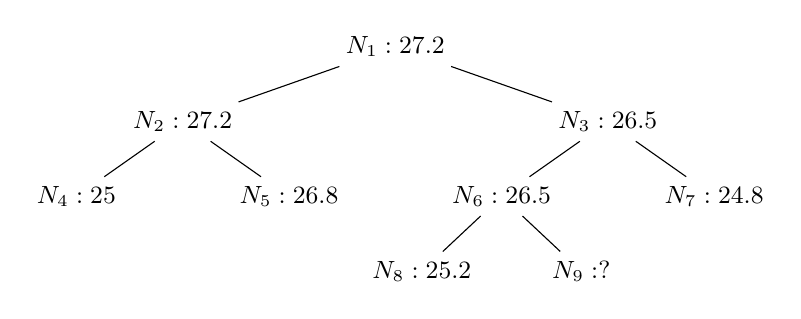
\begin{tikzpicture}[x=1.35cm,y=.95cm,every node/.style={font=\small}]
\node (n1) at (0,0) {$N_1:27.2$};\node (n2) at (-2,-1) {$N_2:27.2$};\node (n3) at (2,-1) {$N_3:26.5$};
\node (n4) at (-3,-2) {$N_4:25$};\node (n5) at (-1,-2) {$N_5:26.8$};\node (n6) at (1,-2) {$N_6:26.5$};\node (n7) at (3,-2) {$N_7:24.8$};
\node (n8) at (.25,-3) {$N_8:25.2$};\node (n9) at (1.75,-3) {$N_9:?$};
\draw (n1)--(n2) (n1)--(n3) (n2)--(n4) (n2)--(n5) (n3)--(n6) (n3)--(n7) (n6)--(n8) (n6)--(n9);
\end{tikzpicture}\end{center}
(a) 从$v_9\le27.2$, $v_9\le26.5$, $v_9=26.5$, $v_9\ge25.2$中选最有信息且必正确者. (b) 给整数最优值$v^*$当前最佳上下界. (c) 依次判断$N_4,N_5,N_7,N_8,N_9$是活跃A、可剪枝F或资料不足NEI.
\end{exercise}
\begin{solution}
官方解答重构. (a) $v_9\le26.5$, 因子节点增加限制而不能提高极大LP值. (b) 叶节点中未剪枝者的最高LP界为$N_5$的26.8, $N_9$也至多26.5. 整数目标值可向下取整, 所以$25\le v^*\le26$. 原解答只援引$N_3$的26.5不能单独界住另一分支, 这里补全$N_5$说明.

(c) $N_4$为F, 因LP最优解已整数; $N_5$为A, 因目标26.8非整数, LP解不是整数方案, 其向下取整界26仍高于25; $N_7$为F, 因24.8低于当前方案; $N_8$为F, 因$\lfloor25.2\rfloor=25$不能改善当前方案; $N_9$为NEI, 只知上界26.5不能判断是否可改善25.
\end{solution}

\begin{exercise}\label{ass:15053-ps6-q2}
作业6第2题. 六投资净现值为$(33,45,25,17,39,23)$, 所需现金为$(10,14,8,6,12,8)$, 现金总限28.

(a) 建0--1投资模型. (b) 以$x=(1,0,0,1,1,0)$、值89为当前方案, 求工作簿的前五节点LP解与值并说明是否剪枝: $N_1$无附加约束, $N_2:x_1=0$, $N_3:x_1=1$, $N_4:x_1=x_2=0$, $N_5:x_1=0,x_2=1$. (c) 解释$N_2,N_3$为何有一个重复$N_1$解, $N_4,N_5$为何有一个重复$N_2$解.
\end{exercise}
\begin{solution}
官方工作簿解答重构并修正$N_3$显示值. (a) $\max33x_1+45x_2+25x_3+17x_4+39x_5+23x_6$, $10x_1+14x_2+8x_3+6x_4+12x_5+8x_6\le28$, $x\in\{0,1\}^6$.

(b) 节点LP以$0\le x\le1$替代二元条件, 结果为
\begin{center}\begin{tabular}{clrl}\toprule
节点&LP产量$(x_1,\ldots,x_6)$&目标&剪枝?\\\midrule
$N_1$&$(1,3/7,0,0,1,0)$&$639/7$&否\\
$N_2$&$(0,1,1/4,0,1,0)$&$361/4$&否\\
$N_3$&$(1,3/7,0,0,1,0)$&$639/7$&否\\
$N_4$&$(0,0,1,0,1,1)$&87&是\\
$N_5$&$(0,1,1/4,0,1,0)$&$361/4$&否\\\bottomrule
\end{tabular}\end{center}
最优LP可以按单位现金净现值由高到低填充, 或用实际求解的对偶价格验证. 原解答工作簿给$N_3$值91.25, 与它列出的产量不符; 正确$639/7=91.2857143$. $N_4$已整数且值87低于89, 可剪; 其他节点的整数上界仍超过89.

(c) $N_1$解本已有$x_1=1$, 增加该等式保留原最优点且缩小可行域, 所以$N_3$重复; $N_2$解本已有$x_2=1$, 同理$N_5$重复. 这也说明对一个已经整数的变量分支未必有效切掉当前LP点.
\end{solution}

\begin{exercise}\label{ass:15053-ps6-q3}
作业6第3题. 对上题模型用割平面, 当前整数方案仍是值89的$(1,0,0,1,1,0)$, 题目说明它确为整数最优.

(a) 解LP, 能否以该结果证明89最优? 若不能继续. (b) 取(a)解中三个正变量的下标$i,j,k$, 加$x_i+x_j+x_k\le2$, 重解并判断能否证明89最优. (c) 再取(b)解中三个正变量, 追加同形割, 重解并判断. 说明所加割为何对整数解有效.
\end{exercise}
\begin{solution}
官方解答重构并补割的有效性. (a) 解$(1,3/7,0,0,1,0)$, LP值$639/7$, 整数上界91仍大于89, 不能证明.

(b) 正变量1、2、5的现金总额36超过28, 三者不能全选, 所以覆盖割$x_1+x_2+x_5\le2$有效. 新LP解为$(1,0,3/4,0,1,0)$, 值90.75, 向下取整界90仍大于89, 不能证明.

(c) 正变量1、3、5现金和30超过28, 追加$x_1+x_3+x_5\le2$. 新LP解为$(1,3/5,3/5,0,2/5,0)$, 值90.6, 界90仍大于89, 也不能证明. 分数LP解本身并非“不可能证明”的理由; 若其目标向下取整已不超过89, 即便分数也可完成证书, 这里是具体界未足够紧. 另外实际枚举64个投资集合可独立验证整数最优为89, 但这不改变题目所问三次LP证书的结论.
\end{solution}

\begin{exercise}\label{ass:15053-ps6-q4}
作业6第4题. 0--1背包目标为$22x_1+10x_2+16x_3+11x_4+18x_5+6x_6$, 容量约束$4x_1+3x_2+7x_3+6x_4+5x_5+8x_6\le15$. 判断下列不等式是否对所有整数可行解有效: (a) $x_1+x_3+x_4\le2$; (b) $x_2+x_3+x_5\le2$; (c) $x_3+x_5\le1$; (d) $x_1+x_2+x_4+x_6\le3$.
\end{exercise}
\begin{solution}
官方解答重构. (a) 有效, 三项全选重量17超过15. (b) 无效, 仅选2、3、5重量恰15而左端3. (c) 无效, 仅选3、5重量12而左端2. (d) 有效, 四项全选重量21超过15, 故至多三项.
\end{solution}

\begin{exercise}\label{ass:15053-ps6-q5}
作业6第5题. 整数规划为$\max(4x_1+3x_2)$, $2x_1+x_2\le11$, $-x_1+2x_2\le6$, $x_1,x_2\ge0$且整数. 令$s_1,s_2$为两约束松弛. LP最优表为
\[
\begin{array}{c|rrrr|r}
 &x_1&x_2&s_1&s_2&\text{右端}\\\hline
-z&0&0&-11/5&-2/5&-133/5\\
x_1&1&0&2/5&-1/5&16/5\\
x_2&0&1&1/5&2/5&23/5
\end{array}
\]
(a) 当$x_1,x_2$整数时, 松弛是否必为整数, 说明理由. (b) 从两条约束行各导出一条Gomory割. (c) 用原变量表示两割, 画可行域与割. (d) 加入必要的割后重解, 最优表如下, $s_3$为新增割松弛. 哪些行可导出Gomory割? 导出并换回原变量.
\[
\begin{array}{c|rrrrr|r}
 &x_1&x_2&s_1&s_2&s_3&\text{右端}\\\hline
-z&0&0&-2&0&-1&-26\\
x_1&1&0&1/2&0&-1/2&7/2\\
s_2&0&0&1/2&1&-5/2&3/2\\
x_2&0&1&0&0&1&4
\end{array}
\]
(e) 画新割, 图解最优方案并判断是否整数最优; 原题提示最终值应为25.
\end{exercise}
\begin{solution}
官方解答重构, 图中原第一约束错标的系数已按题面修正. (a) $s_1=11-2x_1-x_2$, $s_2=6+x_1-2x_2$, 都是整数之差, 故必整数.

(b) 对整数等式$x_B+\sum_ja_jx_j=b$, 向下取整得到$x_B+\sum_j\lfloor a_j\rfloor x_j\le\lfloor b\rfloor$, 再减原等式, 得$\sum_j\{a_j\}x_j\ge\{b\}$. 第一行负系数$-1/5$的分数部分是$4/5$, 不是$-1/5$. 所以两割为
\[
\tfrac25s_1+\tfrac45s_2\ge\tfrac15,\qquad
\tfrac15s_1+\tfrac25s_2\ge\tfrac35.
\]
(c) 代入(a)得到$x_2\le9/2$与$x_2\le4$, 后者更强, 只需加入后者. 原可行多边形的四个顶点为
\[
(0,0),\quad(11/2,0),\quad(16/5,23/5),\quad(0,3).
\]
下图虚线为第一轮两条割, 实线斜割为第二轮; 着色为两轮割后可行域.

\begin{center}\begin{tikzpicture}[x=.8cm,y=.8cm]
\fill[structurecolor!8] (0,0)--(5.5,0)--(4,3)--(3,4)--(2,4)--(0,3)--cycle;
\draw[->] (-.2,0)--(6.3,0) node[right]{$x_1$};\draw[->] (0,-.2)--(0,5.4) node[above]{$x_2$};
\draw (0,0)--(5.5,0)--(3.2,4.6)--(0,3)--cycle;
\draw[dashed] (0,4.5)--(5.5,4.5) node[right]{$x_2\le9/2$};
\draw[dashed,structurecolor] (0,4)--(5.5,4) node[right]{$x_2\le4$};
\draw[thick,structurecolor] (2,5)--(6,1) node[right]{$x_1+x_2\le7$};
\fill (4,3) circle(1.8pt) node[above right]{$(4,3)$};
\node[below] at (5.5,0){$11/2$};\node[left] at (0,3){$3$};
\end{tikzpicture}\end{center}
(d) $x_1$与$s_2$两行右端为半整数, 各自均给$\frac12s_1+\frac12s_3\ge\frac12$, 即$s_1+s_3\ge1$. $x_2$行全为整数, 没有非平凡分数割. 用$s_3=4-x_2$换回, 新割为$x_1+x_2\le7$.

(e) 新LP最优点$(4,3)$, 值25. 将原第一约束乘1、新割乘2相加, 给$4x_1+3x_2\le11+14=25$, 该整数点达到上界. 因为所有割对原整数解有效, 这也证明了原整数规划的最优性.
\end{solution}
